
\vspace{-10ex}%
\rule{\textwidth}{0.3pt}
\vspace{10ex}
 % after-code
 

\section{Layout}
To get a 4 layer board some inintial rules needs to be setup. These parameters are set by the board manufactuer. The minimum measurements are presented in \autoref{PCB_param}

One is the width of the traces. minimum of 6 mils, which equals of 0,1524mm. 
Via diameter: 10
 
\subsection{Landgrid}
The industry standard is always good to aim for, in this case the basic designs are taken from \gls{ipcg}'s design guidline\cite{ipcg}. Whilest these are made for optimal manufacturability the footprints used on the testboard are modified to enable for easier solderability, production and rework if needed. The land grids are made slightly bigger and longer to acheive this. The downside of making the pads larger is that the final board size increases and therefore the size of the land grids requires to be reduced.

\subsection{Easy prototyping}
The components that going to be used in high frequency often comes in tiny packages. This gives the protypability problems with easy ability to solder and use, but the problem is that the best components used in this area of work will be small to fit in small advanced systems. To make a

\section{Structure}
The product is constructed with a number of components, which all have a central role of the final product. They can all be seen in \autoref{fig:sys_dia}. A list of the major components and their function can be seen below:

\begin{itemize}[noitemsep] 
\item \gls{mcu}: The central part of any integrated system, handles all the calculations and the program code.
\item Radio: All the communications with the rest of the world will be handled by the radio, sending on the VHF and UHF band.
\item \gls{imu}: Movement detection is measured with a accelerometer, this to determine if the unit is  in motion or laying still. 
\item \gls{ldo}: A Low-dropout regulator can supply the system with a smoother voltage because no switching is taking place.
\item Hall sensor: The hall sensor is used as a switch for the system by sensing if a magnet is nearby and then turning off the circuit.
\item \gls{rtc}: A real time clock is important to aquire data at a specific set time. It is important that the clock is exact over the whole life of the pruduct.
\end{itemize} 


\begin{figure}[H] 
\centering 
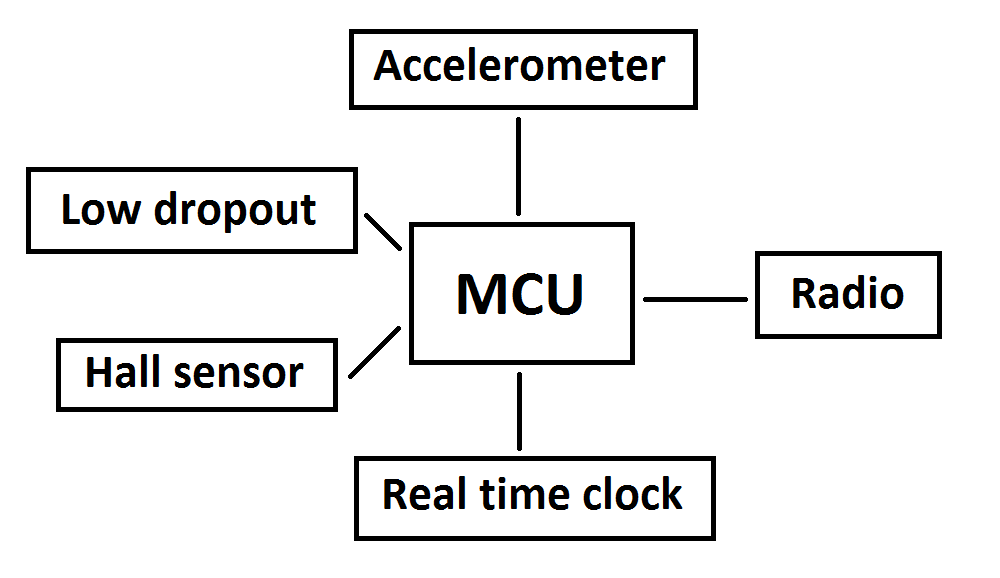
\includegraphics[width=.8\linewidth]{Figures/System_diagram} 
\captionsource{The prototype connection}{Aurthor}
\label{fig:sys_dia} 
\end{figure} 

Each of the components in this project is carfully chosen to get the functionallity and effect that the company is after. To ensure the system works as intended the company have aquired development boards to each of the components. Every components needs to be tested to ensure their induvidial functionallity. Each development board is connected to the micro controllers board. First off the \gls{mcu} have to be set up in a correct way with all it parameters and then the other components could be connected and initilized one after another. The whole connection can be seen. %\autoref{rattbo}.

%\begin{figure}[H] 
%\centering 
%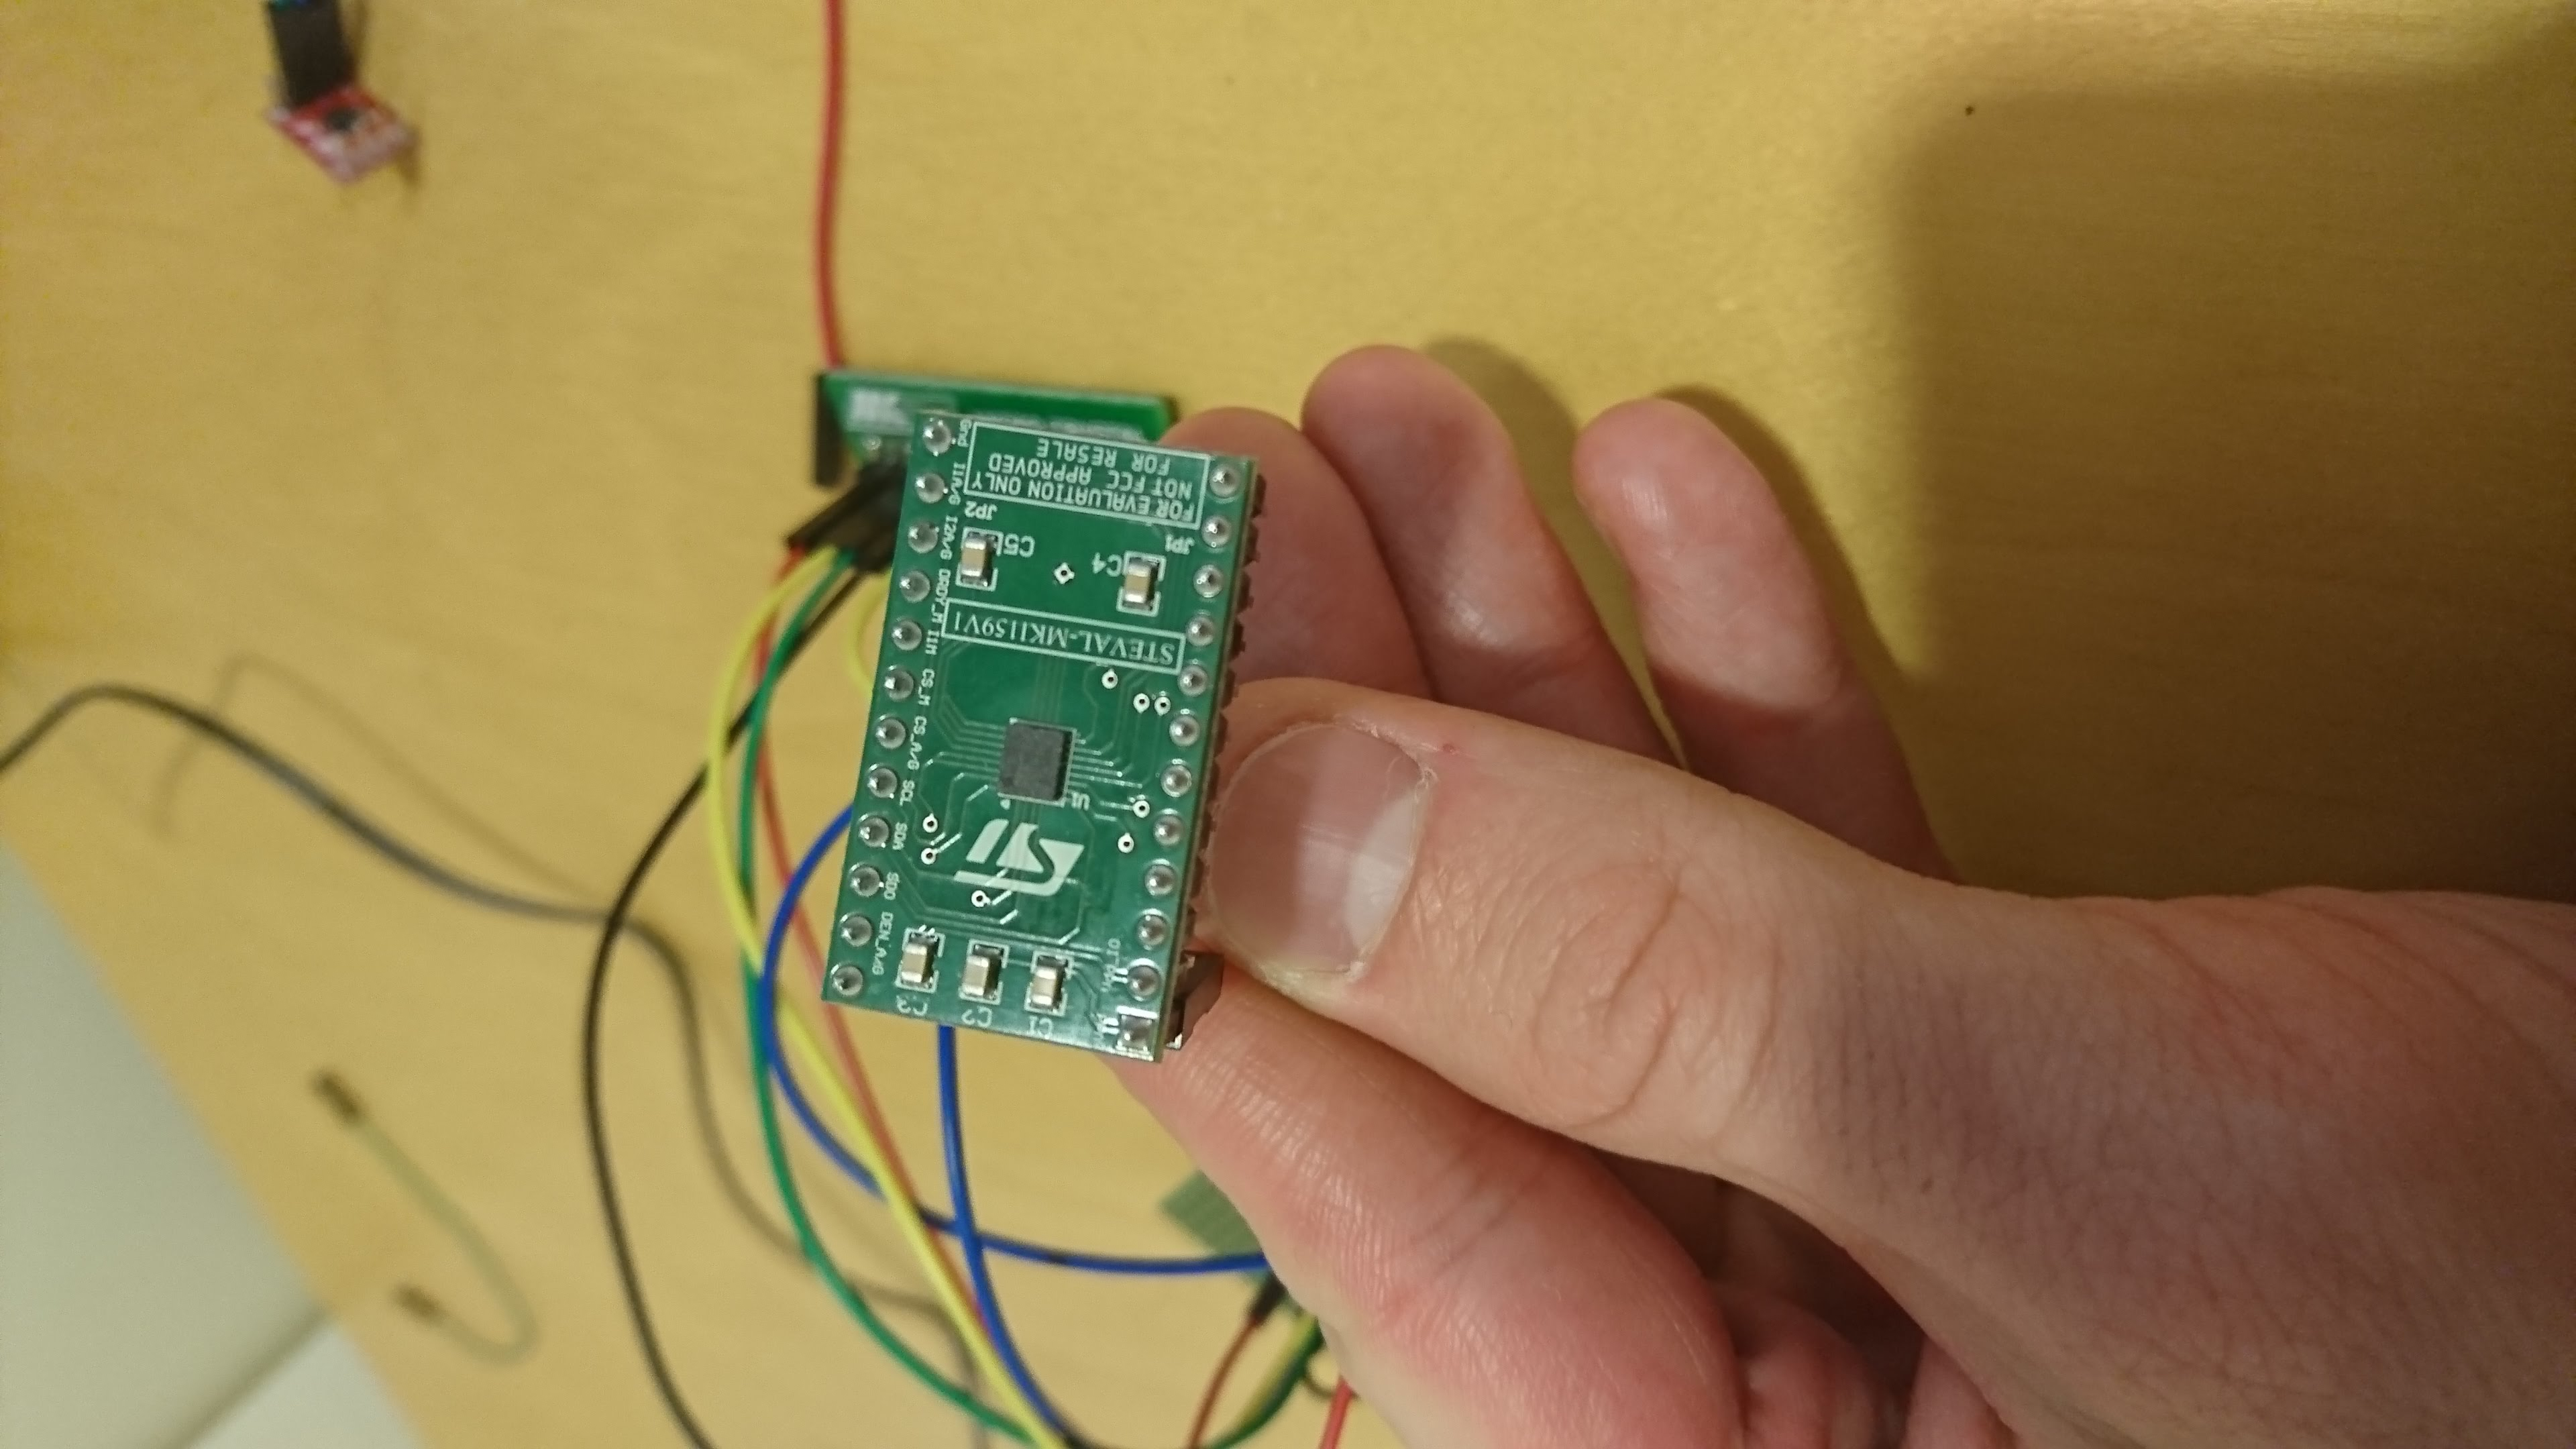
\includegraphics[width=.8\linewidth]{Figures/DSC_0103} 
%\captionsource{The prototype connection}{\url{Aurthor}}
%\label{rattbo} 
%\end{figure} 

%The \gls{mcu} can dtad


\section{MicroController Unit}
The \gls{mcu} used for this project is a processor type that is used by this company many times before and has been chosen to this project for its small size, low power draw, sufficient connections and feautures. The particular processor used is the PIC18LF46K22\cite{pic18}. The version used is one with 40 pins. All the connections avalible are shown in \autoref{Pic18_Pinout}.

\begin{figure}[H] 
\centering 
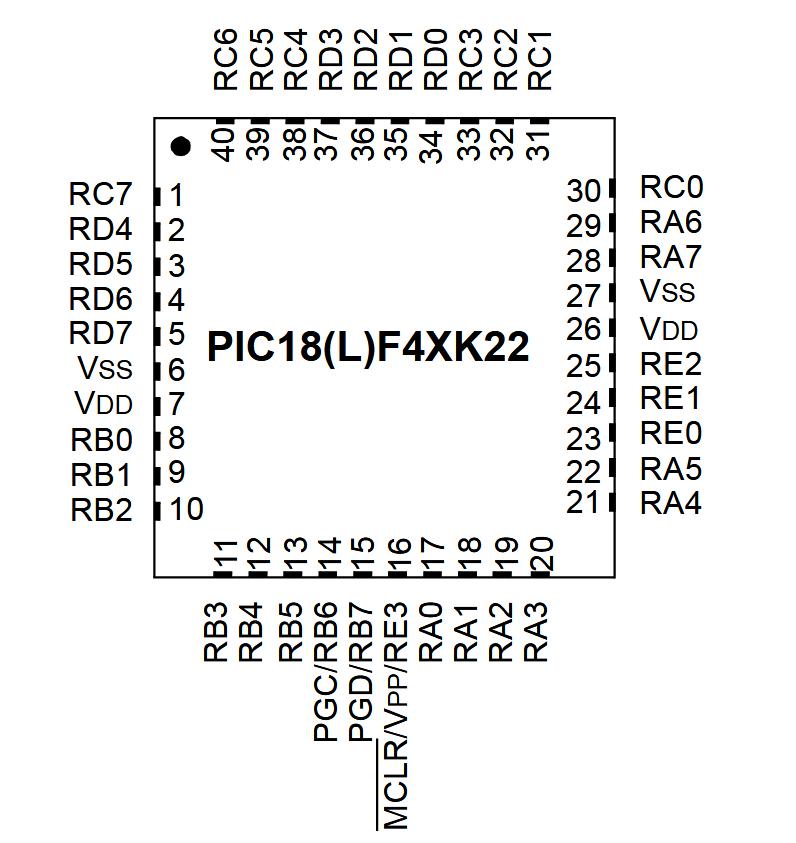
\includegraphics[width=.7\linewidth]{Figures/Pic18_pinout} 
\captionsource{PIC18LF46K22 pinout}{\url{http://ww1.microchip.com/downloads/en/DeviceDoc/40001412G.pdf}}
\label{Pic18_Pinout} 
\end{figure} 

\subsection{Connenctions}

 \subsubsection{Power}
Powering it is done by connnecting the VDD pins to the power net. Connected to ground is the Vss pins on the processor. To ensure the current fed is as smooth as possible capacitors are connected between these two pins. The value of these capacitors are choosen to 100nF.  

\subsubsection{Oscillator}
To operate the \gls{mcu} a clock signal is mandatory, this can be implemented in different ways. Either with the internal High, Medium and Low frequency oscillator or a external one. Where the external rely on a specific circuitry to provide the clock source. Examples of external oscillators are: clock modules, quarts crystal resonators or ceramic resonators and resistor-capacitor circuits. When a circuit is specified to be power efficient the speed of the clock plays a central role. As this product is specified to run on a small battery the speed of the system is kept low to increase the lifetime of the battery. The clock signal is generated from a external temperature compensated Crystal Oscillator (TCXO).


\newpage
\section{Accelerometer} %% Accelerometers
The component used is a 3-axis, ultra-low-power and high performance accelerometer from ST\cite{STacc}. The component is the simplest of IMU's that this manufactorer have and this simplicity makes for a product that is only incorparite one sigle function. 3-axis accelerometer means that it can measure 

\section{Power}
Two voltage connections is apperent on this device, one which is called VDD and the other is called VDD-IO. 

\subsection{Connenctions}


\subsection{Software implementation}



\newpage
\section{Radio}


\subsection{Power}


\subsection{Connenctions}
 In the registers 

\section{Power consumption}
 The total power consumption is calculated by adding the current draw from each induvudual component together.  Different test is conducted to try different modes of the system. One describing the power cunsumption of only the processor. This is done by running it in a infinite loop with all the other components at the circuit powered down or in power down mode. Since the system is not supposed to be active just a small time with a longer power down mode in between the power consumption on the system has to account for a longer time span. The tests is made with a standard scheme used already by the company. The scheme consist of a small radio pulse every second and the system beeing inactive in between these radio pulses. 

